% ===========================================================================
%  TikuOS — TikuKits ML: k-Nearest Neighbors for Embedded Systems
%  Beamer Presentation
% ===========================================================================
\documentclass[aspectratio=169, 10pt]{beamer}

% ---- Theme ----------------------------------------------------------------
\usetheme{Madrid}
\usecolortheme{whale}
\setbeamertemplate{navigation symbols}{}
\setbeamertemplate{footline}{%
  \leavevmode\hbox{%
    \begin{beamercolorbox}[wd=.33\paperwidth,ht=2.5ex,dp=1ex,center]{author in head/foot}%
      \usebeamerfont{author in head/foot}\insertshortauthor
    \end{beamercolorbox}%
    \begin{beamercolorbox}[wd=.34\paperwidth,ht=2.5ex,dp=1ex,center]{title in head/foot}%
      \usebeamerfont{title in head/foot}\insertshorttitle
    \end{beamercolorbox}%
    \begin{beamercolorbox}[wd=.33\paperwidth,ht=2.5ex,dp=1ex,right]{date in head/foot}%
      \usebeamerfont{date in head/foot}\insertshortdate{}\hspace*{2em}%
      \insertframenumber{}/\inserttotalframenumber\hspace*{2ex}
    \end{beamercolorbox}}%
  \vskip0pt%
}

% ---- Packages -------------------------------------------------------------
\usepackage{listings}
\usepackage{graphicx}
\usepackage{hyperref}
\usepackage{booktabs}
\usepackage{multirow}
\usepackage{tikz}
\usetikzlibrary{arrows.meta, positioning, shapes.geometric, calc,
                decorations.pathreplacing, fit}
\usepackage{amsmath}

% ---- Code listing style ---------------------------------------------------
\lstset{
  basicstyle=\ttfamily\scriptsize,
  keywordstyle=\color{blue}\bfseries,
  commentstyle=\color{gray},
  stringstyle=\color{red!70!black},
  showstringspaces=false,
  breaklines=true,
  frame=single,
  rulecolor=\color{black!30},
  backgroundcolor=\color{blue!3},
  tabsize=4,
}
\lstdefinestyle{cstyle}{
  language=C,
  morekeywords={uint8_t,uint16_t,uint32_t,int32_t,int64_t,
                tiku_kits_ml_elem_t,
                TIKU_KITS_ML_OK,TIKU_KITS_ML_ERR_NULL,
                TIKU_KITS_ML_ERR_SIZE,TIKU_KITS_ML_ERR_PARAM,
                TIKU_KITS_ML_KNN_MAX_FEATURES,
                TIKU_KITS_ML_KNN_MAX_SAMPLES,
                TIKU_KITS_ML_KNN_MAX_CLASSES,
                TIKU_KITS_ML_KNN_DEFAULT_K,
                NULL},
}

% ---- Metadata -------------------------------------------------------------
\title[TikuKits ML]{TikuKits ML: $k$-Nearest Neighbors for Embedded Systems}
\subtitle{Simple. Ubiquitous. Intelligence, Everywhere.}
\author[Ambuj Varshney]{Ambuj Varshney \\ \texttt{ambuj@tiku-os.org}}
\date{\today}

% ===========================================================================
\begin{document}

% ---------------------------------------------------------------------------
\begin{frame}
\titlepage
\end{frame}

% ---------------------------------------------------------------------------
\begin{frame}{Outline}
\tableofcontents
\end{frame}

% ===========================================================================
\section{Motivation}
% ===========================================================================

\begin{frame}{Why $k$-NN on MCUs?}
\begin{columns}[T]
\begin{column}{0.48\textwidth}
\begin{block}{Embedded Use Cases}
\begin{itemize}
  \item \textbf{No training phase} --- just store examples
  \item \textbf{Adaptive} --- add new samples on-the-fly
  \item \textbf{Multi-class} --- naturally handles any number of classes
  \item \textbf{Non-parametric} --- no assumptions about data distribution
\end{itemize}
\end{block}

\begin{block}{Constraints}
\begin{itemize}
  \item No FPU (16-bit MSP430)
  \item No heap allocation
  \item Limited RAM (2--8\,KB)
  \item Ring buffer keeps memory bounded
\end{itemize}
\end{block}
\end{column}

\begin{column}{0.48\textwidth}
\begin{center}
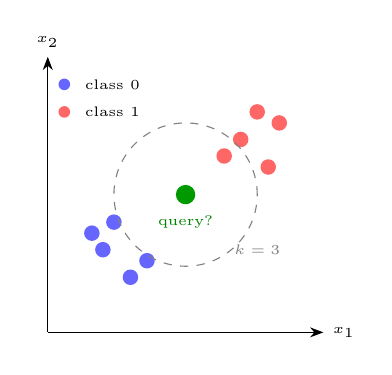
\begin{tikzpicture}[>=Stealth, scale=0.7]
  % Class 0 points (blue)
  \fill[blue!60] (1.0, 1.5) circle (4pt);
  \fill[blue!60] (1.5, 1.0) circle (4pt);
  \fill[blue!60] (1.2, 2.0) circle (4pt);
  \fill[blue!60] (0.8, 1.8) circle (4pt);
  \fill[blue!60] (1.8, 1.3) circle (4pt);

  % Class 1 points (red)
  \fill[red!60] (3.5, 3.5) circle (4pt);
  \fill[red!60] (4.0, 3.0) circle (4pt);
  \fill[red!60] (3.8, 4.0) circle (4pt);
  \fill[red!60] (4.2, 3.8) circle (4pt);
  \fill[red!60] (3.2, 3.2) circle (4pt);

  % Query point
  \fill[green!60!black] (2.5, 2.5) circle (5pt);
  \node[font=\tiny, green!50!black] at (2.5, 2.0) {query?};

  % k=3 circle
  \draw[dashed, gray] (2.5, 2.5) circle (1.3cm);
  \node[font=\tiny, gray] at (3.8, 1.5) {$k=3$};

  % Axes
  \draw[->] (0,0) -- (5,0) node[right] {\tiny $x_1$};
  \draw[->] (0,0) -- (0,5) node[above] {\tiny $x_2$};

  % Legend
  \fill[blue!60] (0.3, 4.5) circle (3pt);
  \node[font=\tiny, right] at (0.5, 4.5) {class 0};
  \fill[red!60] (0.3, 4.0) circle (3pt);
  \node[font=\tiny, right] at (0.5, 4.0) {class 1};
\end{tikzpicture}
\end{center}

\vspace{0.3em}
\begin{alertblock}{Design Goal}
Instance-based classification with \textbf{bounded memory}
via ring buffer, squared Euclidean distance (no \texttt{sqrt}),
and majority voting among $k$ nearest neighbors.
\end{alertblock}
\end{column}
\end{columns}
\end{frame}

% ===========================================================================
\section{Algorithm Theory}
% ===========================================================================

\begin{frame}{$k$-NN Classification}
\begin{columns}[T]
\begin{column}{0.48\textwidth}
\textbf{Distance metric:} Squared Euclidean
\[
  d(\mathbf{a}, \mathbf{b}) = \sum_{j=1}^{n} (a_j - b_j)^2
\]

No \texttt{sqrt()} needed --- ordering is preserved.

\vspace{0.5em}
\textbf{Prediction:}
\begin{enumerate}
  \item Compute distance from query to all stored samples
  \item Select $k$ samples with smallest distance
  \item Majority vote among their labels
  \item Return the most frequent class
\end{enumerate}

\vspace{0.5em}
\textbf{Complexity:} O($N \times F$) per query,\\
where $N$ = stored samples, $F$ = features.
\end{column}

\begin{column}{0.48\textwidth}
\begin{block}{Ring Buffer Storage}
When the sample buffer is full, new samples \textbf{overwrite} the oldest.
This creates a sliding-window effect --- the classifier adapts to recent data.

\vspace{0.3em}
\begin{center}
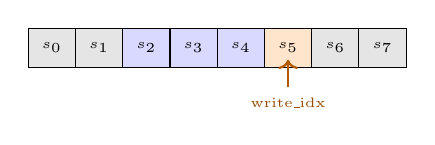
\begin{tikzpicture}[
    cell/.style={draw, minimum width=0.6cm, minimum height=0.5cm,
                 font=\tiny\ttfamily}
  ]
  \node[cell, fill=gray!20] at (0, 0) {$s_0$};
  \node[cell, fill=gray!20] at (0.6, 0) {$s_1$};
  \node[cell, fill=blue!15] at (1.2, 0) {$s_2$};
  \node[cell, fill=blue!15] at (1.8, 0) {$s_3$};
  \node[cell, fill=blue!15] at (2.4, 0) {$s_4$};
  \node[cell, fill=orange!20] at (3.0, 0) {$s_5$};
  \node[cell, fill=gray!20] at (3.6, 0) {$s_6$};
  \node[cell, fill=gray!20] at (4.2, 0) {$s_7$};

  \draw[->, thick, orange!70!black] (3.0, -0.5) -- (3.0, -0.15);
  \node[font=\tiny, orange!60!black] at (3.0, -0.7) {write\_idx};
\end{tikzpicture}
\end{center}
\end{block}

\vspace{0.3em}
\begin{block}{Overflow Safety}
Differences are cast to \texttt{int64\_t} before squaring:
$2^{31} \times 2^{31} = 2^{62} < 2^{63}$.
Accumulation over 8 features stays within \texttt{int64\_t}.
\end{block}
\end{column}
\end{columns}
\end{frame}

% ===========================================================================
\section{Data Structure}
% ===========================================================================

\begin{frame}[fragile]{The \texttt{tiku\_kits\_ml\_knn} Structure}
\begin{columns}[T]
\begin{column}{0.48\textwidth}
\begin{lstlisting}[style=cstyle,
  title={ml/classification/tiku\_kits\_ml\_knn.h}]
struct tiku_kits_ml_knn {
    tiku_kits_ml_elem_t
        data[TIKU_KITS_ML_KNN_MAX_SAMPLES]
            [TIKU_KITS_ML_KNN_MAX_FEATURES];
    uint8_t
        labels[TIKU_KITS_ML_KNN_MAX_SAMPLES];
    uint16_t n_samples;
    uint16_t write_idx;
    uint8_t  n_features;
    uint8_t  k;
};
\end{lstlisting}

\textbf{Memory footprint:}\\
$32 \times 8 \times 4 + 32 + 2 + 2 + 1 + 1 = 1062$ bytes.\\
All statically allocated.
\end{column}

\begin{column}{0.48\textwidth}
\begin{lstlisting}[style=cstyle,
  title={Configuration macros}]
/* Max features per sample */
#ifndef TIKU_KITS_ML_KNN_MAX_FEATURES
#define TIKU_KITS_ML_KNN_MAX_FEATURES 8
#endif

/* Max stored samples */
#ifndef TIKU_KITS_ML_KNN_MAX_SAMPLES
#define TIKU_KITS_ML_KNN_MAX_SAMPLES 32
#endif

/* Max output classes */
#ifndef TIKU_KITS_ML_KNN_MAX_CLASSES
#define TIKU_KITS_ML_KNN_MAX_CLASSES 8
#endif

/* Default k */
#ifndef TIKU_KITS_ML_KNN_DEFAULT_K
#define TIKU_KITS_ML_KNN_DEFAULT_K 3
#endif
\end{lstlisting}
\end{column}
\end{columns}
\end{frame}

% ===========================================================================
\section{API Reference}
% ===========================================================================

\begin{frame}[fragile]{Complete API}
\begin{table}
\centering
\small
\begin{tabular}{@{}lp{8cm}@{}}
\toprule
\textbf{Function} & \textbf{Description} \\
\midrule
\texttt{tiku\_kits\_ml\_knn\_init(knn, nf, k)}
  & Initialize with \texttt{nf} features, $k$ neighbors \\
\texttt{tiku\_kits\_ml\_knn\_reset(knn)}
  & Clear all stored samples \\
\texttt{tiku\_kits\_ml\_knn\_add(knn, x, label)}
  & Add sample (ring buffer, overwrites oldest when full) \\
\midrule
\texttt{tiku\_kits\_ml\_knn\_predict(knn, x, \&result)}
  & Classify by majority vote of $k$ nearest \\
\midrule
\texttt{tiku\_kits\_ml\_knn\_set\_k(knn, k)}
  & Change $k$ at runtime \\
\texttt{tiku\_kits\_ml\_knn\_get\_k(knn)}
  & Get current $k$ value \\
\texttt{tiku\_kits\_ml\_knn\_count(knn)}
  & Number of stored samples \\
\bottomrule
\end{tabular}
\end{table}

\vspace{0.3em}
\begin{alertblock}{Minimum Data Requirement}
\texttt{predict()} requires at least $k$ stored samples.
Returns \texttt{ERR\_SIZE} if fewer than $k$ samples are available.
Labels must be in range $[0, \text{MAX\_CLASSES})$.
\end{alertblock}
\end{frame}

% ===========================================================================
\section{Examples}
% ===========================================================================

\begin{frame}[fragile]{Example 1: Temperature Zone Classification}
\begin{lstlisting}[style=cstyle,
  title={examples/example\_ml\_knn.c --- 3 zones with k=3}]
struct tiku_kits_ml_knn knn;
uint8_t result;

tiku_kits_ml_knn_init(&knn, 1, 3);   /* 1 feature, k=3 */

/* Add calibration samples: cold(0), normal(1), hot(2) */
int32_t cold[] = {100, 120, 150, 170, 180};
int32_t norm[] = {220, 240, 250, 260, 280};
int32_t hot[]  = {320, 340, 350, 360, 380};

uint8_t i;
for (i = 0; i < 5; i++) {
    tiku_kits_ml_knn_add(&knn, &cold[i], 0);
    tiku_kits_ml_knn_add(&knn, &norm[i], 1);
    tiku_kits_ml_knn_add(&knn, &hot[i],  2);
}

/* Classify new readings */
int32_t query1 = 140;
tiku_kits_ml_knn_predict(&knn, &query1, &result);   /* result = 0 (cold) */

int32_t query2 = 330;
tiku_kits_ml_knn_predict(&knn, &query2, &result);   /* result = 2 (hot) */
\end{lstlisting}
\end{frame}

% ---------------------------------------------------------------------------
\begin{frame}[fragile]{Example 2: Gesture Recognition}
\begin{columns}[T]
\begin{column}{0.52\textwidth}
\begin{lstlisting}[style=cstyle,
  title={2-D accelerometer: tap/shake/tilt}]
struct tiku_kits_ml_knn knn;
uint8_t result;

tiku_kits_ml_knn_init(&knn, 2, 3);

/* Tap: small X, large Y spike */
tiku_kits_ml_elem_t tap1[] = {5, 50};
tiku_kits_ml_elem_t tap2[] = {-3, 55};
tiku_kits_ml_knn_add(&knn, tap1, 0);
tiku_kits_ml_knn_add(&knn, tap2, 0);

/* Shake: large X, large Y */
tiku_kits_ml_elem_t shk1[] = {40, 45};
tiku_kits_ml_elem_t shk2[] = {-35, 50};
tiku_kits_ml_knn_add(&knn, shk1, 1);
tiku_kits_ml_knn_add(&knn, shk2, 1);

/* Tilt: moderate X, small Y */
tiku_kits_ml_elem_t tlt1[] = {20, 5};
tiku_kits_ml_elem_t tlt2[] = {25, -3};
tiku_kits_ml_knn_add(&knn, tlt1, 2);
tiku_kits_ml_knn_add(&knn, tlt2, 2);

/* Classify new gesture */
tiku_kits_ml_elem_t q[] = {3, 48};
tiku_kits_ml_knn_predict(&knn, q,
                         &result);
/* result = 0 (tap) */
\end{lstlisting}
\end{column}

\begin{column}{0.44\textwidth}
\begin{center}
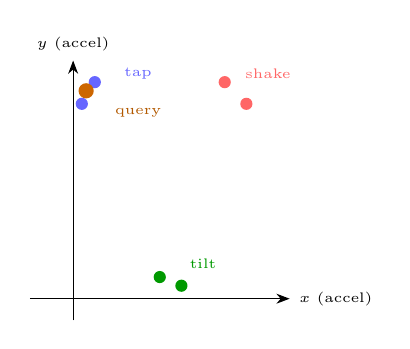
\begin{tikzpicture}[>=Stealth, scale=0.55]
  \draw[->] (-1,0) -- (5,0) node[right] {\tiny $x$ (accel)};
  \draw[->] (0,-0.5) -- (0,5.5) node[above] {\tiny $y$ (accel)};

  % Tap cluster
  \fill[blue!60] (0.5, 5.0) circle (4pt);
  \fill[blue!60] (0.2, 4.5) circle (4pt);
  \node[font=\tiny, blue!60] at (1.5, 5.2) {tap};

  % Shake cluster
  \fill[red!60] (4.0, 4.5) circle (4pt);
  \fill[red!60] (3.5, 5.0) circle (4pt);
  \node[font=\tiny, red!60] at (4.5, 5.2) {shake};

  % Tilt cluster
  \fill[green!60!black] (2.0, 0.5) circle (4pt);
  \fill[green!60!black] (2.5, 0.3) circle (4pt);
  \node[font=\tiny, green!60!black] at (3.0, 0.8) {tilt};

  % Query
  \fill[orange!80!black] (0.3, 4.8) circle (5pt);
  \node[font=\tiny, orange!70!black] at (1.5, 4.3) {query};
\end{tikzpicture}
\end{center}

\vspace{0.5em}
\begin{block}{Dynamic $k$}
Change $k$ at runtime with \texttt{set\_k()}:
\begin{itemize}
  \item Small $k$ (1--3): noisy but responsive
  \item Large $k$ (5--7): smoother, slower
\end{itemize}
\end{block}
\end{column}
\end{columns}
\end{frame}

% ===========================================================================
\section{Test Suite}
% ===========================================================================

\begin{frame}{Test Cases Overview}
\begin{table}
\centering
\small
\begin{tabular}{@{}clp{7cm}@{}}
\toprule
\textbf{\#} & \textbf{Test Function} & \textbf{What It Verifies} \\
\midrule
1 & \texttt{test\_kits\_ml\_knn\_init}
  & Proper initialization, parameter validation \\
2 & \texttt{test\_kits\_ml\_knn\_simple}
  & 1-D classification with 3 classes \\
3 & \texttt{test\_kits\_ml\_knn\_two\_features}
  & 2-D classification \\
4 & \texttt{test\_kits\_ml\_knn\_k1}
  & Nearest-neighbor ($k=1$) classification \\
5 & \texttt{test\_kits\_ml\_knn\_change\_k}
  & Runtime $k$ change via \texttt{set\_k()} \\
6 & \texttt{test\_kits\_ml\_knn\_overflow}
  & Ring buffer overwrites oldest samples \\
7 & \texttt{test\_kits\_ml\_knn\_negative}
  & Negative feature values handled correctly \\
8 & \texttt{test\_kits\_ml\_knn\_reset}
  & Reset clears all stored samples \\
9 & \texttt{test\_kits\_ml\_knn\_null\_inputs}
  & All functions reject NULL with ERR\_NULL \\
\bottomrule
\end{tabular}
\end{table}
\end{frame}

% ===========================================================================
\section{Summary}
% ===========================================================================

\begin{frame}{Summary}
\begin{columns}[T]
\begin{column}{0.48\textwidth}
\begin{block}{What We Built}
\begin{itemize}
  \item Instance-based $k$-NN classifier
  \item Ring buffer for bounded memory
  \item Squared Euclidean distance (no \texttt{sqrt})
  \item Majority voting with tie-breaking
  \item $\sim$1\,KB state (default 32 samples $\times$ 8 features)
\end{itemize}
\end{block}

\begin{block}{Key Design Choices}
\begin{itemize}
  \item \texttt{int64\_t} distance accumulation
  \item Ring buffer for sliding-window adaptation
  \item Runtime-adjustable $k$ value
  \item Up to 8 classes supported
\end{itemize}
\end{block}
\end{column}

\begin{column}{0.48\textwidth}
\begin{block}{Use Cases}
\begin{itemize}
  \item Temperature zone classification
  \item Gesture recognition (accelerometer)
  \item Adaptive monitoring with new samples
  \item Multi-class sensor classification
\end{itemize}
\end{block}

\begin{block}{Files}
\scriptsize
\begin{tabular}{@{}lp{4.5cm}@{}}
Header: & \texttt{ml/classification/tiku\_kits\_ml\_knn.h} \\
Source: & \texttt{ml/classification/tiku\_kits\_ml\_knn.c} \\
Tests: & \texttt{tests/ml/test\_kits\_ml\_knn.c} \\
Example: & \texttt{examples/example\_ml\_knn.c} \\
\end{tabular}
\end{block}
\end{column}
\end{columns}
\end{frame}

% ---------------------------------------------------------------------------
\begin{frame}{Thank You}
\begin{center}
\Large\textbf{TikuKits ML: $k$-Nearest Neighbors}\\[0.5em]
\normalsize Integer-Only Machine Learning for Physical AI Endpoints\\[1.5em]

\begin{tabular}{rl}
  Repository: & \url{https://github.com/tikuos/tikuOS} \\
  License:    & Apache 2.0 \\
  Common:     & \texttt{tikukits/ml/tiku\_kits\_ml.h} \\
  Header:     & \texttt{tikukits/ml/classification/tiku\_kits\_ml\_knn.h} \\
  Source:     & \texttt{tikukits/ml/classification/tiku\_kits\_ml\_knn.c} \\
  Tests:      & \texttt{tikukits/tests/ml/test\_kits\_ml\_knn.c} \\
  Examples:   & \texttt{tikukits/examples/example\_ml\_knn.c} \\
\end{tabular}
\end{center}
\end{frame}

\end{document}
